\chapter{LITERATURE REVIEW}
\section{Introduction}
A literature review is a critical synthesis of existing research and scholarly resources relevant to a specific field of study, as suggested by \parencite{walker2010systematic}. In the context of Bayesian Network modeling for operational risk, this literature review will explore published academic articles and journals, industry guidelines, and other relevant resources that address the framework for quantifying and validating causal relationships in operational risk management. By examining prior research on using Bayesian Networks to model operational risk and establish a framework for quantifying and validating causal relationships, this chapter aims to highlight the current state of knowledge and identify gaps that the present study seeks to address. The literature review will objectively summarize past studies, methodologies, and findings while critically assessing their contributions to the field. This will help establish a theoretical foundation for the study and clarify the rationale for employing Bayesian Network modeling to improve operational risk management practices. Through this process, the chapter will demonstrate how integrating causal modeling can enhance the framework's effectiveness for quantifying and validating causal relationships in operational risk management.
\subsection{Operational Risk}
Operational risk has emerged as a major focus within the financial sector, largely because of its influence on the routine functioning of economic institutions. This growing interest has drawn the attention of industry professionals, regulators, and academics alike. Studies have shown that a key challenge in this field remains the absence of a commonly accepted definition of operational risk across different expert communities. For this study, we use the definition proposed by the \textcite{bcbs2020operationalrisk}, and the one adopted in the Accord is” the risk of direct or indirect loss resulting from inadequate or failed internal processes, people and systems or from external events, and this definition includes legal risk”.  It should be noted that according to this accord, this definition was developed for all financial institutions, Banks, and insurance companies concerning specific risk elements. According to the revised Basel Committee report, “legal risk includes but is not limited to, exposure to fines, penalties, or punitive damages resulting from supervisory actions, as well as private settlements.

The table \ref{tab:risks} in the next page outlines a structured Operational Risk Taxonomy, categorizing risks into Level 1 (broad categories) and Level 2 (detailed sub-risks). It covers people, fraud, technology, process failures, and conduct. This classification helps firms systematically identify, assess, and manage operational risks, ensuring compliance with regulatory standards like Basel and enhancing risk control and reporting.

\begin{table}[H]
\centering
\caption{Level 1 and Level 2 Operational Risks}
\label{tab:risks}
\resizebox{\textwidth}{!}{%
\begin{tabular}{|l|l|}
\hline
\textbf{Level 1 Risks} & \textbf{Level 2 Risks} \\
\hline
\multirow{4}{*}{People} 
 & Breach of employment legislation \\
 & Breach of regulatory requirements \\
 & Ineffective employment relations \\
\hline
\multirow{3}{*}{External Fraud} 
 & Third party/vendor fraud \\
 & Agent/ Broker/ Intermediary fraud \\
 & First party Fraud \\
\hline
\multirow{3}{*}{Internal Fraud} 
 & Internal fraud committed against the organisation \\
 & Internal Fraud committed against Customer \\
 & Internal Fraud committed against Clients \\
\hline
\multirow{3}{*}{Physical Security and Safety} 
 & Damage to the organisation's physical properties \\
 & Injury to employees/affiliates outside the workplace \\
 & Damage to or injury to public assets \\
\hline
Business Continuity 
 & Inadequate business continuity planning or event management \\
\hline
\multirow{5}{*}{Transaction or Processing and Execution} 
 & Execution failure relating to clients and products \\
 & Execution failure relating to securities and collateral \\
 & Execution failure relating to the third party \\
 & Execution failure relating to internal operations \\
 & Change execution failure \\
\hline
\multirow{3}{*}{Technology} 
 & Hardware failure \\
 & Software failure \\
 & Network failure \\
\hline
\multirow{12}{*}{Conduct} 
 & Insider trading \\
 & Improper market practices \\
 & Post service failure \\
 & Client Mistreatment \\
 & Client Account Mismanagement \\
 & Improper distribution/ marketing \\
 & Improper product or service design \\
 & Breach of code of conduct \\
 & Employee misbehaviour \\
\hline
\end{tabular}%
}
\end{table}

\subsection{An interconnected operational risk landscape }
An increasing interconnectivity of the operational risk landscape is rapidly changing the way risks are viewed and assessed. The recently published report by ORX shows that among actively participating members, emerging operational risks are fully interconnected, where the boundaries between individual risk and associated internal and external risk factors cannot be easily separated. The Bayesian Belief Network presents a promising way to tackle this through the use of a direct cyclic graph, a local Markov property, to assess and drive a better understanding and visibility of vulnerabilities, interconnections, and concentrations of risk (often undertaken as part of operational resilience efforts). The interconnectedness between individual risks creates a combined risk profile that exceeds the sum of its parts. The report shows that in the context of geopolitical uncertainty and economic strain, it is surprising that cybercrime ranks as the top emerging risk.

The Reserve Bank of Zimbabwe (RBZ), Financial Stability reports produced from 2022 to 2024 agree with the ORX global report that cybercrime is ranked as the highest risk indicator. The integration and adoption of more sophisticated AI machines, business software, and do-it-yourself portals have significantly increased the cases of cyberattacks in many companies as they are exposed to the risks associated with rapid technology advancement. Organizations must take this opportunity of rapid growth in technology to harness these innovations, which help in managing risks from outdated banking systems amongst other related automated systems. Concerns about risks from outdated machines, systems, and increased business disruptions are amplified by heavy reliance on a complex network of third-party providers, particularly concentrated around cloud service providers, creating potential systemic risks. At the same time, regulatory pressures are intensifying the focus on these critical areas.
\subsection{Operational Risk surfaces expand as a trade-off to rapid digitalization}
Businesses must digitalize not only to seize new opportunities but also to stay competitive. The speed of change requires institutions to carefully balance the risks of hurried change management, accumulating technical debt, outdated legacy systems, and security issues introduced by new technologies against the risk of falling behind. The rapid pace of technology transformation from old systems to AI and automated systems is also complicating the cost-benefit analysis related to the control environment. Ultimately, this ongoing transformation increases the exposure of institutions to risks in ways that are difficult to predict and evaluate. In a rapidly changing risk environment, Bayesian networks allow firms to understand how different risks influence each other, quantify the probability of cascading failures, and update risk assessments as new information emerges. This dynamic modeling helps businesses anticipate potential vulnerabilities across their digital transformation, operational processes, and third-party dependencies, enabling proactive risk management.
\begin{figure}[H]
    \centering
    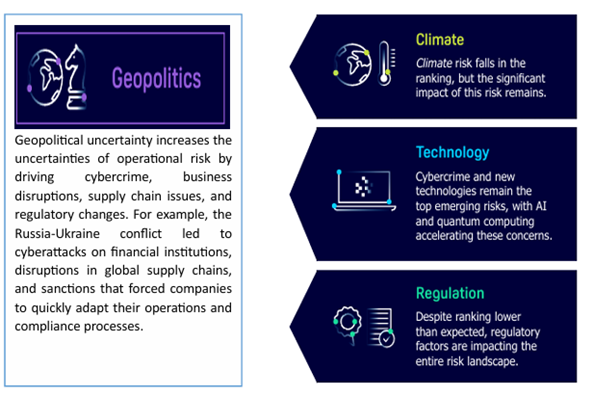
\includegraphics[width=0.75\linewidth]{External Environment.png}
    \caption{A rapidly evolving external environment }
    \label{fig: External environment}
\end{figure}
Figure \ref{fig: External environment} describes various factors contributing to operational risk, including geopolitical uncertainty, climate change, technological advancements, and regulatory shifts. Geopolitical instability, such as the Russia- Ukraine conflict, heightens cyber threats, disrupts supply chains, and forces businesses to adapt to evolving regulations. While climate risks have declined in ranking, their impact remains significant. Emerging technologies, particularly AI and quantum computing, continue to escalate cyber risks, whereas regulatory changes affect the broader risk landscape. Together, these factors increase operational risk complexity, necessitating proactive risk management strategies for business resilience.
\subsection{Percentage of global total loss falling in each loss size bin}
\begin{figure}[H]
    \centering
    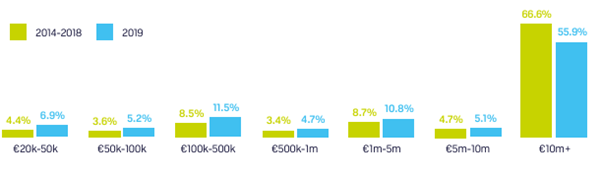
\includegraphics[width=1\linewidth]{Global Total Loss 1.png}
    \caption{The distribution of total monetary losses }
    \label{fig: Total monetary losses}
\end{figure}

\begin{figure}[H]
    \centering
    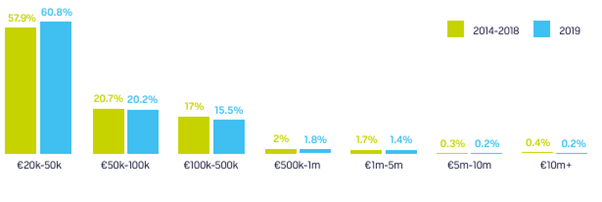
\includegraphics[width=1\linewidth]{Global Total Loss 2.png}
    \caption{The total percentage of the number of events }
    \label{fig: Percentages}
\end{figure}
Figure \ref{fig: Total monetary losses} illustrates the distribution of total monetary losses across various loss-size categories. The data shows that high-value loss events exceedingly more than USD 10 million account for the largest share of overall loss, often exceeding 50\% of the total. In contrast, smaller loss bins (e.g., below \$50,000.00) represent a relatively minor portion of total losses. This suggests that while smaller events may occur frequently, a few very large incidents drive the majority of the financial impact.

Figure \ref{fig: Percentages} above focuses on the percentage of the number of events occurring in each loss-size category. Unlike Figure \ref{fig: Total monetary losses}, it reveals that the majority of incidents fall into smaller loss bins (for instance, under \$20,000.00 or between \$20,000.00 and \$50,000.00). Large-scale risk events above 10 million remain relatively rare., This typically constitutes a small fraction of the total events. This discrepancy between Figures 7 and 8 underscores a key operational risk insight: Most loss incidents are relatively minor, but a small number of severe events account for the greatest financial impact.

The ORX data indicates a growing trend in cumulative losses and a growing number of operational risk events, with high-severity incidents driving most of the total financial impact \parencite{orx2024lossdata}. Meanwhile, smaller losses are much more frequent, yet represent a smaller portion of the aggregate loss. This pattern highlights the need for robust modeling techniques that can capture both frequent low-level incidents and rare but high-impact events. In the literature, Bayesian Belief Networks (BBNs) have gained attention as a powerful tool for quantifying operational risk, as they allow the integration of empirical data and expert judgment to model dependencies among risk factors, estimate the probability of extreme events, and ultimately support more effective risk mitigation strategies.

How to construct a Bayesian Network diagram that establishes a relationship between the necessary operational risk attributes is not yet fully resolved. As previously stated in \textcite{basel2021principles}, Banks must develop, implement, and maintain an operational risk management framework that is fully integrated into the institution’s overall risk management processes. Therefore, we need to clarify to what extent the quantifying methodologies permit the construction and validation of a model that considers the main features of all operational risks. The Basel Committee on Banking Supervision reviewed the Operational risk management framework adopted by an individual institution and stated that a Bank will depend on a range of factors, including the bank’s nature, size, complexity, and risk profile. The losses generated by the operational risk are identified and connected under the international standards for the seven-event types, internal fraud, external fraud, employment practices and the safety of the working place, the clients, the products, and the commercial practices; the tangible assets loss, the activity rupture and the inadequate systems functioning and the process execution, the delivery, and management  (Barbu et al, 2010). 

\section{Empirical Literature}
\subsection{Bayesian Network Structure and Operational Risk }

The quantification of operational risk under the regulatory standards Basel II and Solvency II is a challenging task; many financial institutions adopt a Loss Distribution Approach to estimate this risk capital charge (Klugman, Panjer and Willmot, 2008), Operational Value-at-Risk,\textcite{sanford_operational_2015}, and Scenario analysis Approach, \textcite{andersen2016causal}. These approaches require a combination of internal and external data, as well as expert opinions. The Bayesian Network scenario to estimate the parameters of the risk frequency and severity distributions has been proposed by \parencite{aquaro_bayesian_2009}, to provide insights into the estimation of operational risk.

Bayesian network structure can be defined as a probabilistic graphical model that explicitly captures the known conditional dependence with directed edges in a graph model \parencite{janson2019bayesian}, with all the missing connections defining the conditional independencies in the model. \textcite{ramamurthy2005operational} described the Bayesian Network as a quantitative or causal probabilistic network that helps, model, measure, and manage operational risk before knowledge of the causal risk factors and probabilistic reasoning. Bayesian Networks provide a useful tool to visualize the probabilistic model for a domain, review all of the relationships between the random variables, and reason about causal probabilities for scenarios given available evidence. According to Janson, Bayesian network models capture both conditionally dependent and conditionally independent relationships between random variables. 

\textcite{guney2019introduction}, defined the Bayesian Network, or Belief Network as a Probabilistic Graphical Model (PGM) that represents conditional dependencies between random variables through a Direct Acyclic Graph (DAC) which can be applied in many fields, particularly for this research we are mainly focused on the operational risks which are being faced in all financial institutions. More precisely, Bayesian networks are directed acyclic graphs that allow efficient and effective representation of the joint probability distribution over a set of random variables as alleged by \textcite{fenton2008using} and \textcite{leo2020managing}. Each vertex in the graph represents a random variable, edges represent direct correlations between the variables, and the network encodes the conditional independence statements where each variable is independent of its non-descendants in the graph given the state of its parents. These independencies are then exploited to reduce the number of parameters needed to characterize a probability distribution and to efficiently compute posterior probabilities. Probabilistic parameters are encoded in a set of tables, one for each variable, in the form of local conditional distributions of a variable given its parents. 

\textcite{pearl1988probabilistic} claims that the Bayesian Theory contains information about causal probability relationships between variables and is used for decision-making in managing risk. The causal probability relationships in a Bayesian Theorem are represented by nodes which depict the variables and direct arcs which represent the conditional relationship in the form of a direct acyclic graph. Bayesian Networks are suitable for modeling operational risk because they can represent complex causal relationships between risk factors and quantify uncertainties probabilistically. This theory supports the integration of expert knowledge and data, allowing for a comprehensive analysis even when data is scarce or incomplete \parencite{alexander2006bayesian}. BNs enable scenario analysis and inference by updating probabilities based on new evidence, which is essential for stress testing and dynamic risk assessment. More precisely, their structure facilitates model validation, as the causal dependencies can be compared with empirical data to ensure consistency and accuracy \parencite{cowell_modeling_2007}.

Financial databases usually constitute high noise and nonlinearity levels, making it difficult to train deep learning models like Deep Belief Networks, Bayesian Belief Networks, and Convolutional Neural Networks \parencite{liu_risk_2021}.

\textbf{High noise:}
\begin{equation}
x_i = x_i^{\text{true}} + \varepsilon_i, \quad \varepsilon_i \sim \mathcal{N}(0, \sigma^2)
\end{equation}
where \( \varepsilon_i \) represents Gaussian noise with high variance \( \sigma^2 \)] and \( \eta_i \) is additional noise.
\vspace{10pt}

\textbf{Nonlinearity:}
The underlying function \( f: \mathbb{R}^d \rightarrow \mathbb{R} \) relating \( x_i \) and \( y_i \) is highly nonlinear, i.e.,
\begin{equation}
y_i = f(x_i) + \eta_i
\end{equation}

Bayesian Belief Network models require substantial amounts of training data, but financial data offer a more complex, limited dataset, which makes it more challenging to validate the models. The application of advanced sophisticated financial risk models in the financial industry presents several advantages. BBN can handle large-scale high-dimensional data in both industries, the Health, Financial, and manufacturing industries as illustrated by \textcite{zhao_data_2024}, and unearth hidden patterns and trends, aiding in identifying potential risk factors and correlations. BBN models present strong generalisation capabilities that are adaptable to operational risk management needs across different types and domains (Yazdi et al., 2024). 

In addition, BBN and Deep Network analysis can automate risk identification and quantification, determining the minimum capital reserve for banks, and insurance industries \parencite{buddiga_advancing_2022}. The integration of artificial intelligence in operational risk management has increasingly led to rapid expansion of new perspectives and more advanced tools with powerful data processing and analytical capabilities across various industries. Amongst the newly adopted data analytical tools, is machine learning through AI, deep learning, and big data analytics Shi et al.(2025) and \textcite{feng2024deep}. These analytical tools offer a promising solution to the rapid advancement in technology towards risk management. The world is rapidly moving towards new tech, which concurrently comes with its potential limitations to the industry, as cyber attackers find loopholes in outdated banking systems, and phishing schemes become prominent in underdeveloped nations.

This literature presents the opinions of various authors regarding the Bayesian Network analysis of operational risk.\textcite{hager_knowledge_2010}, suggested the Bayesian Network as a powerful tool for quantitative analysis of the causal relationships determining the loss severity. This framework has been suggested to solve the problem of scarce data by data-driven models and also improving scenario-based methods. They constructed a causal model based on the mechanisms that determine the loss size for a specific event and further modeled the root causal drivers for the identified loss determinants. They found that the Bayesian model framework provides a formalized model structure and scientifically sound theoretical basis for scenario modeling.


\textcite{shevchenko2009implementing} applied the Loss distribution approach for operational risk, which allows to take into account expert judgment and parameter uncertainty into account, modeling dependency from their observations the Bayesian framework is convenient for combining different data sources (internal data, external data, and expert opinions) and to account for the relevant uncertainties. It has been noted that accurate quantification of the dependencies between ORs is a difficult task with many challenges to be resolved. Therefore, many aspects of the LDA may require further research. 

Therefore, a study carried out by \textcite{tudor_operational_2017} reviewed the usual ways of quantifying operational risk in Loss Distribution Approach (LDA) models. In their findings, they recommended that we clarify to what extent the quantifying methodologies permit the construction of a model that considers the main features of all operational risks in any financial institution.  A research study by \textcite{sanford_operational_2015} developed an operational risk modeling tool using a Bayesian network to capture causal relationships between risk factors and losses. The research provides a prediction of operational loss distributions and, and Operational Value for-risk management. Continuous variables were approximated using static discretization, though more sophisticated methods were used. From their findings, the Bayesian enhances risk prediction, adaptability, and communication in operational risk management. Another related research, by \textcite{liu_bayesian_2022} addressing the key aspect of operational risk shows that the Bayesian framework enables effective risk management. The research employs vine copulas within a Bayesian framework to model dependencies between different types of data breaches, whilst using public data sets, the study finds that the optimal vine structure provides more conservative value-at-risk estimates than other models. 

A case study conducted by \textcite{universidad_panamericana_operational_2017} focused on quantifying capital requirements for operational risk in a Mexican financial institution using an advanced Bayesian inference model has revealed that operational risk can be estimated with 95\% confidence even with limited data, with a positive correlation between expert expectations and operational risk levels. Their primary objective was to develop a robust operational risk measurement framework, in cases where historical loss data is insufficient. The study employs a conjugated Poisson-Gamma distribution, integrating expert interviews to estimate parameters, and utilizes Monte Carlo simulations to model expected losses. Furthermore, the frequency and severity of losses fluctuate dynamically as the risk threshold is approached. These insights highlight the importance of model assumptions and expert input in risk quantification. The proposed methodology serves as a foundation for developing risk mitigation strategies, enabling financial institutions to proactively manage operational risk and minimize potential losses.

Bayesian network models have been and continue to be applied to diverse problem domains, particularly in the financial sector industry. Other statisticians argue that operational risk managers are not interested in the characterization or categorization of operational risks, but rather in the frequency and severity of operational losses \parencite{hager2010knowledge}, which gives the number of monetary losses incurred. The research analyzed operational losses to understand their causes and impacts, using data warehouses for low-impact, high-frequency losses, and qualitative methods for rare, high-impact events. The key findings indicate that storing loss data and using Management information system reports helps identify key risk drivers, while qualitative approaches like self-assessments foster a culture of risk awareness. This approach is relevant to operational risk management as it supports decision-making by providing insights into frequent losses and focuses on qualitative strategies for rare risks.

The Bayesian Network can incorporate the elements of the Advanced Measurement approach, which include internal data, external data, scenario analysis, and factors reflecting the business environment and the control system in a simple. \textcite{martinez2016analysis} applied the Bayesian approach to manage Operational Risk in the international banking sector, incorporating real-world elements like specific risk distributions and expert opinions. As preferred by other scholars, Bayesian Networks offer advantages over other models by integrating internal and external data, scenario analysis, and causal relationships. They provide a more realistic framework for calculating operational risk, highlighting the Bayesian Network's effectiveness in Operational Risk management.

\textcite{tudor_operational_2017}, developed a Bayesian Network framework for quantifying and validating operational risk key factors, and in their findings, they picked some limitations in the current operational risk management. Their main findings depict a lack of rigorous backward-looking validation of forecasts and simulations. They advised that estimations used for risk quantification should be validated with econometric tests and that the actual outcomes should be compared to predict risks. Other Authors argue that the absence of detailed historical data on multiple causes affects the ability to perform thorough post-event analysis, making the simulation process a potential operational risk. Automation and technology, such as blockchain, could improve data collection and standardization, enabling better causal relationship analysis and risk quantification. To enhance Bayesian network models for operational risk, incorporating comprehensive data on causal relationships and using tools like process diagrams could help validate and quantify risks more effectively.

In addition to the above, operational risk is significant in all financial institutions and it’s a major critical concern for financial institutions, as it can lead to substantial losses resulting from failures in internal processes, or external events. Operational risk is hard to quantify, given the presence of heavy-tailed loss distribution (Martin et al, 2020), and the lack of data usually for low-frequency and high-impact losses (Acharyya et al, 2023).

Despite regulatory advancements, such as the Basel II and Basel III Accords, operational risk modeling remains challenging due to the complexities in identifying, quantifying, and validating the interconnected causal relationships between risk factors. While traditional methods like the Loss Distribution Approach (LDA) are widely used, they do not fully quantify the key operational risk factors. Amongst the more sophisticated methods developed are linear models such as time series, econometric, and empirical actuarial models. These models tend to rely on historical data to predict future values based on past trends.  Operational Risk losses often exhibit fat-tailed distributions, which means extreme losses would occur more frequently than would be predicted by linear models. Therefore, the relationship between variables in operational risks is non-linear and complex, making it difficult to model accurately using linear models. However, despite extensive research on operational risk, the significance for quantifying and validating key operational risk factors remains unclear. 

\textcite{zhao_data_2024} traditional risk management methods rely heavily on historical data and statistical models, and are no longer effective in the highly volatile and fast-changing financial sector. He developed a law risk prediction model called WBIF, which integrates Bidirectional Long Short-Term Memory (BiLSTM) and Fully Convolutional Networks (FCN), with parameter optimization performed using the Whale Optimization Algorithm (WOA). The study focused on improving the accuracy and adaptability of risk prediction in financial markets. The main findings show that the WBIF model reduced the Mean Absolute Error (MAE) by 51.73\% on the UCI machine learning dataset and improved accuracy by 12\% on the Kaggle credit card fraud detection dataset. The study concluded that deep learning models optimized with advanced algorithms like WOA can significantly enhance risk prediction accuracy, surpassing traditional statistical approaches.

A study carried out by \textcite{eze2024harnessing} asserts that operational risk management is crucial for organizations to protect themselves from disruptions, financial losses, and reputational harm. The author used a methodology that examined the role of data analytics in enhancing operational risk management to study how organizations can leverage advanced analytics techniques to manage risks more effectively. The main findings show that data analytics enables organizations to extract actionable insights from large data sets, allowing them to identify, assess, and mitigate risks proactively. The study ends by concluding that by integrating data analytics into operational risk management, organizations can strengthen their operational resilience and enhance long-term business sustainability.

Bayesian Network (BN) modeling presents a promising framework for addressing this gap by providing a probabilistic, causal structure that links risk factors in a visual node map. BNs allow for overcoming these hurdles as they combine qualitative data from experts and relevant quantitative data. However, key challenges persist in constructing and validating such models, particularly in defining the relationships between risk attributes, quantifying probabilities, and ensuring the model's practical application is valid in day-to-day risk management \parencite{dimaio2022integration}. Financial institutions struggle to fully integrate these models into their operational risk frameworks beyond regulatory compliance.

All these methods discussed above were employed by various authors in trying to quantify the causal relationship between the key operational risk factors under different cases. From the analysis of this literature, there is still a need for further research to fill in the gaps and to develop the Bayesian network framework for operational risk, which can be used to quantify and validate the causal relationship \parencite{liu_bayesian_2022}. It has been noticed that many studies lack rigorous validation methods, especially backward-looking validations using econometric tests. Furthermore, the integration of real-world data and expert opinion is often limited, which reduces the models’ ability to capture the complications of key operational risks \parencite{cheng2025deep}. However, few studies address the incorporation of dynamic risk environments and the development of new technologies like deep learning and machine learning, which could enhance Bayesian Network models for better real-time risk quantification and validation.

\section{Technical Literature}
\subsection{Introducing the Bayesian network framework}
A Bayesian network is a statistical model that relates the marginal distributions of “causal” factors, or “attributes” of a risk, to its multivariate distribution. By definition, Bayesian Networks are a type of Probabilistic Graphical Model that uses Bayesian inferences for probability computations. As discussed above, it represents a set of variables and its conditional probabilities with a Directed Acyclic Graph (DAG). They are primarily suited for considering an event that has occurred and predicting the likelihood that any of the possible known causes is the contributing factor.\\
\textbf{Definition (Bayesian network)}

A Directed Acyclic Graph (DAG) where $G$ is called an \emph{I-map} of a probability distribution $P$ if every conditional independence displayed on $G$ through the rules of d-separation is valid in $P$. More simply, for every $X$, $Y$, and $Z$,
\begin{equation}
(X \perp_G Y \mid Z) \Rightarrow (X \perp_P Y \mid Z)
\end{equation}

where $(X \perp_G Y \mid Z)$ indicates d-separation of $X$ and $Y$ given $Z$, and $(X \perp_P Y \mid Z)$ denotes conditional independence in the underlying distribution $P$.

$G$ is a Bayesian network if and only if it is a \emph{minimal I-map} of $P$, i.e., no edges can be removed from $G$ without violating the I-map property.

This definition states that the structure implies a set of conditional independence relations among the variables involved, and all of them must be valid. It is interesting to note that the implication does not go both ways; nodes that are d-connected (i.e., not d-separated) in the graph $G$ are not necessarily dependent in the underlying distribution $P$.

Therefore, a completely connected DAG, for example, is always an I-map (since it implies no independencies), although it may not be a valid Bayesian Network according to the definition (if it is not minimal).

As illustrated in the diagram below, we can obtain the Joint Probability Distribution (JPD) with conditional probabilities by using the relationships specified by the Bayesian Network. Each node in the graph represents a random variable, and the arcs (directed edges) represent the relationships between the nodes. 

The network uses Bayes’ rule to propagate through the network, allowing the distributions at all nodes to be quantified, given the prior probabilities and conditional probabilities for all nodes. Each node in the graph corresponds to a unique random variable, and the edges represent probabilistic dependencies among them. 

A Bayesian Network (BN) is a Directed Acyclic Graph (DAG), meaning all edges are directed and there are no cycles—i.e., it is not possible to start at any node, follow the direction of the edges, and return to the starting point.

\begin{figure}[H]
    \centering
    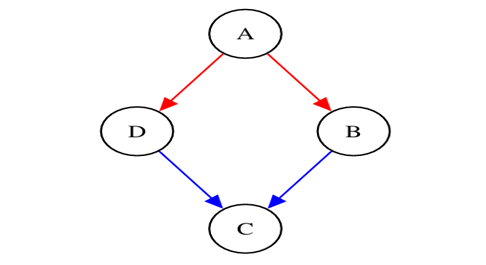
\includegraphics[width=1\linewidth]{DAG Sample 1.png}
    \caption{A diagram showing the relationships between nodes A, B, C, and D}
    \label{fig:DAG 1}
\end{figure}

In the above diagram, A, B, C, and D, are four random variables represented by nodes in the network of the graph. Node A is the parent of B, and C is B’s child. Node C is independent of A. These visuals are easy to understand for stakeholders, aiding in linking risk measurement and management within an institution.

Bayesian Networks satisfy the Local Markov Property (Pavan, 2024), where a node is conditionally independent of its non-descendants given its parents. 
For example, \[P(D\mid A, B) = P(D\mid A)\] since D is independent of B. This simplifies the Joint Distribution and leads to the concept of a Markov Random Field, a random field that follows Markov properties. 

\textcite{sohan2024conditional}, described the Conditional Probability of event A as the probability that event A will occur given that another event B has already happened. Conditional probability is the likelihood of an event occurring, given that another specific event has occurred.
 Based on probability theory, the conditional probability of an event A given event B is denoted as P(A/B). This measures the probability of event A when event B is known to have occurred, effectively reducing the sample space to only those outcomes where event B is true (Shankar, 2021). The formula defines the conditional probability. 
The conditional probability of event \( A \) given event \( B \) is defined as:
\begin{equation}
P(A \mid B) = \frac{P(A \cap B)}{P(B)}
\end{equation}
Here, \( P(A \cap B) \) represents the probability of both events A and B co-occurring (the intersection of A and B), and \( P(B) \) is the probability of event B occurring.

Bayes’ theorem, named after the Reverend Thomas Bayes, helps in determining the probability of an event based on the occurrence of another related event. In the context of this study, Bayes’ theorem is used to update our beliefs about the likelihood of a series of events or risks based on new information. Operational risks—those arising from failures in internal processes, systems, or external events—often rely on conditional probabilities that evolve as new data or incidents occur. Bayes’ formula exists for both events and random variables. Bayes’ theorem formulas are derived from the definition of conditional probability and can be applied to both discrete events \( A \) and \( B \), and continuous random variables \( X \) and \( Y \).

\begin{figure}[H]
    \centering
    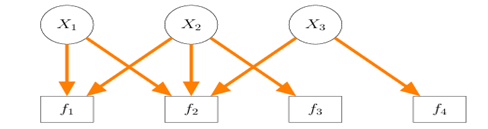
\includegraphics[width=1\linewidth]{DAC Sample 2.png}
    \caption{Conditional Probability and Bayesian Theorem}
    \label{fig: Bayesian Theorem}
\end{figure}

BNs describe the joint probability distribution over a set of variables, given the conditional dependencies/independencies contained in the graphical structure. Given a Bayesian Network (BN) with a set of variables: \( X = (X_1, X_1 \ldots X_n) \), where each variable \( X_i \) may depend on a subset of other variables, its “parents” in the network, denoted as \( \text{pa}(X_i) \), we can write the conditional probability distribution of each variable given its parents as \( P(X_i \mid \text{pa}(X_i)) \). The full joint probability distribution of the network is then the product of all these conditional probabilities. Mathematically, this is expressed as:

\begin{equation}
P(X_1, X_2, \ldots, X_n) = \prod_{j=1}^{n} P(X_i \mid x_{\text{Parents}(i)})
\end{equation}

\begin{equation}
= \prod_{j=1}^{n} P(X_i \mid \text{pa}(x_i))
\end{equation}

This formula is powerful because it allows us to compute the joint probability distribution of the entire set of variables by considering only the local conditional dependencies defined in the BN. This reduces the complexity of inference and calculation significantly, especially in large networks, by leveraging conditional independence relationships.


\section*{Explanation of Each Term}

\begin{enumerate}
    \item \( P(X_i \mid \text{pa}(X_i)) \): The probability of a variable \( X_i \) given its parents, i.e., the variables it directly depends on. If a variable \( X_i \) has no parents, then \( P(X_i \mid \text{pa}(X_i)) \) simplifies to \( P(X_i) \), since it has no dependencies.

    \item \( \prod_{j=1}^{n} \): The product notation signifies that we multiply the conditional probabilities for all variables in the network, from \( X_1 \) to \( X_n \).

    \item \( X = (X_1, X_2, X_3, \ldots, X_n) \): A collection of \( n \) random variables where each \( X_i \) belongs to a domain and is associated with factors \( f_1, f_2, \ldots, f_m \), and each \( f_i(x) \geq 0 \).

    \item The weight \( w(x) \) is defined as:
    \begin{equation}
    w(x) = \prod_{j=1}^{m} f_i(x)
    \end{equation}
    This represents the product of all factors evaluated at a particular configuration \( x \).
\end{enumerate}

\section*{Definition}

Therefore, by definition, let \( X = (X_1, \ldots, X_n) \) be a set of random variables. A Bayesian Network (BN) is a directed acyclic graph (DAG) that specifies a joint distribution over \( X_1 \) as a product of local conditional distributions, one for each node. 

\[
X = (X_1, X_2, X_3, \ldots, X_n)
\]

Considering \( n \) random variables \( X_1, X_2, X_3, \ldots, X_n \), a Bayesian Network would have \( n \) nodes where node \( j \) (with \( 1 \leq j \leq n \)) corresponds to the random variable. The joint probability of random variables in the BN would then be defined as:

\begin{equation}
\text{def} = \prod_{j=1}^{n} P(X_i \mid \text{Parents}(X_i))
\end{equation}

This defines a large joint distribution in a modular way, one variable at a time. The graph captures what other variables a given variable depends on. Then we specify a local conditional distribution for variable \( X_i \), which gives an assumption \( x_{\text{Parents}(i)} \) to its parents. Then the joint distributions are simply defined to be the product of all the local conditional distributions together. 

Bayes’ theorem allows the determination of posterior probabilities based on prior probabilities and the likelihood of an event given the causes.

\textbf{Prior probability}: Represents the strength of belief in a hypothesis or parameter value before data is gathered. It may also represent prior knowledge or information about an event \parencite{mikkola2024prior}.

\textbf{Posterior probability}: Represents how the investigator’s beliefs have changed after the data is considered. It is the probability of an event occurring given that another event has occurred \parencite{hart2022posterior}.

\subsection{Prior Distribution (Unconditional Probability Distribution) }
When using the Bayesian network for calculations, one should master well the Prior Bayesian formula and apply it with flexibility. The given formula below can be used to simplify the calculation of probability distribution in Bayesian Networks. The prior distribution of a variable \(X_i\) in a Bayesian Network is computed by marginalizing all other variables in the network. It is given by the following formula

\begin{equation}
p(X_i)=\sum_{F_x} \left[ p(X_i \mid pa(X_i)) \cdot p(F_x) \right]
\end{equation}
\begin{itemize}
    \item \( p(X_i) \) is the prior distribution of \( X_i \).
    \item \( F_x \) is the set of all other variables in the network.
    \item \( \text{pa}(X_i) \) denotes the parent nodes of \( X_i \).
    \item \( p(X_i \mid \text{pa}(X_i)) \) is the conditional probability of \( X_i \) given its parents.
    \item \( p(F_x) \) is the joint probability distribution of the other variables in the network.
\end{itemize}

\section*{Posterior Distribution (Conditional Probability Distribution)}

The posterior distribution represents the updated probability of a variable given some evidence \( E \). It is computed using Bayes' Theorem:

\begin{equation}
p(X_i \mid E) = \frac{p(E \mid X_i) \cdot p(X_i)}{p(E)}
\end{equation}

Where:
\begin{itemize}
    \item \( p(X_i \mid E) \) is the posterior distribution of \( X_i \) given the evidence \( E \).
    \item \( p(E \mid X_i) \) is the likelihood of the evidence \( E \) given \( X_i \), which is computed by summing over the conditional probabilities of the evidence given the parents of \( X_i \).
    \item \( p(X_i) \) is the prior distribution of \( X_i \) (as computed earlier).
    \item \( p(E) \) is the marginal likelihood of the evidence, computed by summing over all possible configurations of \( X_i \) and the other variables in the network:
    \begin{equation} 
    p(E) = \sum_{X_i} p(E \mid X_i) \cdot p(X_i)
    \end{equation}
\end{itemize}

\section*{Loss Distribution Approach (LDA)}

The Loss Distribution Approach is a statistical technique that estimates the distribution of losses based on historical data. The LDA assumes that operational losses are driven by two independent factors, the frequency and the severity of the event. The frequency is the number of loss events that occur in a given period, such as a year. The LDA works like this, we list all the things that could go wrong for a company, such as Fraud, system glitches, execution errors, and legal issues. Then we figure out how likely each event is and how much money it will cost. Then create a sort of overall Bayesian map showing the possible losses and decide how much money it needs to have on hand (kind of like a safety net) to cover unexpected financial loss from the potential issues. This could be a way to address what-ifs in the business world. The LDA captures tail risk, provides a quantitative measure of the operational risk exposure, and can accommodate different operational risk losses \parencite{hadley_selection_2019}. The mathematical expression below simplifies the loss distribution approach that banks use to set the Net capital requirement to offset the loss in the event of an unexpected business interruption. Using notation adapted from \textcite{embrechts2011modelling}, loss events are denoted as; 
\begin{equation}
\{X_{t,n}^{b,l}\}, \quad \text{for } t = 1, 2, \dots, 8; \quad l = 1, 2, \dots, 7; \quad n = 1, 2, \dots, N_t^{b,l}
\end{equation}
Where \( X_{t,n}^{b,l} \) is a random variable for the loss severity of the \(n^{\text{th}}\) loss event occurring in fiscal year \(t\) for the business line \(b\) and the event type \(l\), and \( N_t^{b,l} \) is a random random variable for the number of losses occurring in fiscal year \(t\) for business line \(b\) and event type \(l\). Thus, \( S_{T+1} \) is a random variable for firm-wide annual operational loss for next fiscal year and can be calculated as
\begin{equation}
S_{T+1} = \sum_{b=1}^8 \sum_{l=1}^7 \sum_{n=1}^{N_{T+1}^{b,l}} X_{T+1,n}^{b,l} = \sum_{b=1}^8 \sum_{l=1}^7 L_{T+1}^{b,l} 
\end{equation}
Where \( L_{T+1}^{b,l} \) is the annual loss for business line \(b\) and event type \(l\) in year \( T + 1 \). The goal of the LDA is to estimate the distribution of \( S_{T+1} \) via simulation and calculate RC as the 99.9\% quantile of this estimated distribution. There are two sources of randomness in \( S_{T+1} \), the loss frequency and the loss severity. The loss frequency, \( N_{T+1}^{b,l} \), is a discrete random variable for the number of losses occurring next fiscal year in business line \(b\) and event type \(l\). And the loss severity, \( X_{T+1,n}^{b,l} \), is a non-negative, continuous random variable as defined in (1). When calculating RC, we follow two common assumptions:

\begin{enumerate}
    \item \( N_t^{b,l} \) are independent of \( X_{t,n}^{b,l} \) for a given business line \(b\), event type \(l\), and year \(t\);
    \item \( \{X_{t,n}^{b,l}\} \) for \( t = 1,2,\dots,8; l=1,2,\dots,7; n=1,2,\dots,N_t^{b,l} \) are independent and identically distributed for a given business line \(b\), and event type \(l\).
\end{enumerate}

To estimate loss severity distributions, losses mapped to a given event type may be combined across business lines to produce an operational risk category (ORC), which is the level at which the banks model generates a separate distribution to estimate potential losses \parencite{hadley_selection_2019}.
Risk Severity is the extent of the damage to the institution, its people, and its goals and objectives resulting from a risk event occurring. The severity of risk is the degree of damage that could result from a risk event. Operational risk severity is a rating that businesses assign to risk based on their potential impact and likelihood of occurring. The severity of risk can be categorized as low, medium, or high. This allows risk managers to determine how much attention and resources should be devoted to managing risk.

\section*{Operational Loss Distribution}

Operational Loss Distribution models the aggregate financial losses resulting from operational risk events within a specified period, typically annually. The modeling process involves two key components: the frequency distribution, which estimates the number of loss events, and the severity distribution, which assesses the magnitude of each loss \parencite{cohen_estimating_2024}. By selecting appropriate statistical distributions for frequency (e.g., Poisson or Negative Binomial) and severity (e.g., Lognormal, Weibull, Gamma, or Generalized Pareto), financial institutions can simulate the overall loss profile through Monte Carlo methods or analytical convolution techniques \parencite{hadley_selection_2019}. This approach enables the estimation of the aggregate loss distribution, from which risk metrics such as Value-at-Risk (VaR) or Expected Shortfall (ES) can be derived. 

These metrics are crucial for determining the regulatory capital required to absorb extreme but plausible losses, with institutions often targeting high quantiles (e.g., the 99.9th percentile) to comply with regulatory standards. The Loss Distribution Approach (LDA), commonly employed under the Basel II and III frameworks, provides a structured methodology for quantifying operational risk. However, its effectiveness depends on the quality of loss data, appropriate model selection, and the consideration of tail events, ensuring that risk is neither underestimated nor overestimated, thus supporting sound capital planning and operational resilience.

\section*{Bayesian Network parameters determination}

Bayesian Network parameters to be quantified include state probabilities for root nodes and quantifying conditional probabilities (Conditional Probability Tables (CPT) or Conditional Probability Functions (CPF)) which model the probabilistic relationship between connected nodes. A quantified Bayesian Network can perform forward or backward inference, including diagnostic analyses with various inference algorithms based on Bayes’ theorem \parencite{moradi_integration_2022}.

Inference algorithms are divided into exact (message-passing, conditioning, junction tree, symbolic probabilistic inference, etc.) and approximate inferences (stochastic sampling, search-based algorithm, and loopy belief propagation algorithm). Learning parameters in a Bayesian network involves determining the conditional probability table for each node, assuming the network structure is already established. Traditionally, experts would estimate these probabilities using prior knowledge, but this approach can deviate significantly from empirical data. Modern techniques emphasize data-driven learning of these parameters, which enhances accuracy for further analysis. A key characteristic of Bayesian networks is their ability to directly represent real-world relationships rather than only focusing on reasoning processes \parencite{Chaoyu2020}.

\section*{Learning the Bayesian Parameters}

Learning the Bayesian parameters given a fixed network structure is a mammoth task, in statistics, and it requires substantial knowledge about Bayesian Statistical inference. According to the study on Learning Bayesian Network Model Structure from Data by \textcite{Margaritis2003}, priori distribution is assumed over the parameters of the local pdfs before the data are used. The conjugacy of a prior distribution is beneficial because it ensures that the posterior distribution belongs to the same family as the prior, but with updated hyperparameters \parencite{Dearden2013}. 

For multinomial distributions, the conjugate prior comes from the Dirichlet Family. Denoting the probability of each bin, \( p_{ijk}, k=1,\dots,r \) in the local probability density function of the variable \( X_i \) for the parent configuration \( pa_{ij} \), the Dirichlet distribution over these parameters is expressed by;

\begin{equation}
p_{ijk}, k=1,\dots,r | G = \text{Dir}(\alpha_{ij1}, \alpha_{ij2}, \dots, \alpha_{ijr}) = \frac{\Gamma(\alpha_{ij}) \prod_{k=1}^{r_i} p_{ijk}^{\alpha_{ijk}}}{\prod_{k=1}^{r_i} \Gamma(\alpha_{ijk})}
\end{equation}
Where \( \alpha_{ijk} \) are its hyperparameters and \( \alpha_{ij} = \sum_{k=1}^{r} \alpha_{ijk} \)

Assuming local and global parameter independence, the distribution over the set of parameters \( p \) of the entire BN is 
\begin{equation}
\Pr(p | G) = \prod_{i=1}^n \prod_{j=1}^{q_i} \frac{\Gamma(\alpha_{ij})}{\prod_{k=1}^{r_i} \Gamma(\alpha_{ijk})} \prod_{k=1}^{r_i} p_{ijk}^{\alpha_{ijk} - 1} 
\end{equation}

Conditional on the dataset \( D \), the posterior probability over the parameters is also a member of the Dirichlet family, since it is conjugate before the multinomial. It is

\begin{equation}
p_{ijk} | G,D = \text{Dir}(N_{ij1} + \alpha_{ij1}, N_{ij2} + \alpha_{ij2}, \dots, N_{ijr} + \alpha_{ijr})
\end{equation}

And 

\begin{equation}
\Pr(p | G) = \prod_{i=1}^n \prod_{j=1}^{q_i} \frac{\Gamma(\alpha_{ij} + N_{ij})}{\prod_{k=1}^{r_i} \Gamma(N_{ijk} + \alpha_{ijk})} \prod_{k=1}^{r_i} p_{ijk}^{N_{ijk} + \alpha_{ijk} - 1}
\end{equation}

Where \( N_{ij} \) represents the number of samples that fall into the \(k\)-th bin of the probability density function (pdf) for the variable \( X_i \), given that its parent nodes are in the \(j\)-th configuration (this is known as the sufficient statistic for that pdf). When using this distribution to predict the value of any quantity \( Q(X_1,X_2,\dots,X_n) \) that depends on the variables in the domain, you compute the prediction by averaging over all possible values of the (unknown) parameters—essentially integrating out the uncertainty in the parameters to make the prediction more robust.

\begin{equation}
\Pr(Q(X_1,X_2,\dots,X_n) | G,D) = \int Q(X_1,X_2,\dots,X_n) \Pr(P | G,D) dp
\end{equation}

More often, for reasons of convenience, the maximum likelihood (ML) parameters are used instead of the entire distribution. The ML for \( p_{ijk} \) is 
\begin{equation}
p_{ijk} = \frac{\alpha_{ijk} + N_{ijk}}{\alpha_{ij} + N_{ij}}
\end{equation}

Also, for convenience, especially in cases where data are abundant, the hyperparameters are ignored \( \alpha_{ijk} \ll N_{ijk} \) and the fraction \( \frac{N_{ijk}}{N_{ij}} \) is used instead. 

\section*{Learning the Structure: Score-based Methods}

One of the most popular methods of inducing BNs from data, especially for pdf estimation, is the score-based approach. The process assigns a score to each candidate BN, typically one that measures how well that BN describes the data set \( D \). Assuming a structure \( G \), its score is

\[
\text{Score}(G,D) = \Pr(G | D)
\]

in other words, the posterior probability of \( G \) given the data set. A score-based algorithm attempts to maximize this score. Computation of the above can be cast into a more convenient form by using Bayes’ law:

\begin{equation}
\text{Score}(G,D) = \Pr(G | D) = \frac{\Pr(D | G) \Pr(G)}{\Pr(D)}  
\end{equation}

To maximize this, we need only maximize the numerator, since the denominator does not depend on \( G \). There are several ways to assess \( \Pr(G) \) from prior information. 

To calculate \( \Pr(D | G) \), the Bayesian approach averages over all possible parameters, weighing each by its posterior probability as discussed above. As we mentioned above, score-based algorithms attempt to optimize this score, returning the structure \( G \) that maximizes it.

\section{Markov Chain Monte Carlo (MCMC)}
Markov Chain Monte Carlo (MCMC) is a group of algorithms that use Markov Chains to draw samples from probability distributions that provide elegant solutions to the Bayesian problems of prediction and model choice \parencite{gilks2001markov}. MCMC is based on a random walk to produce a sequence of models from the model space. The Markov chain aspect is that a new model is generated conditional on the previous one, and the process is independent of how the previous model was arrived at.

According to \textcite{karandikar2006mcmc}, and \textcite{gallagher2009markov}, the basis of MCMC is that we choose a model from some a priori specified range of the model parameters, and then propose a new model, conditional on the current model. From the proposed model, we then decide whether to replace or not to replace the current model with the proposed one. MCMC is particularly useful when direct sampling from a distribution is difficult or impossible, such as in high-dimensional spaces or when the distribution is complex \textcite{koop1997bayesian}. MCMC algorithms construct a Markov chain whose equilibrium distribution approximates the target probability distribution, meaning that the chain eventually settles into a distribution resembling the desired one. 

The causal discovery and Bayesian inference framework was developed by \textcite{annadani2023bayesdag}, \textcite{mclachlan2024approach}, and  \textcite{gilks2001markov}, and the framework addresses computational challenges in joint inference over the combinatorial space of DAGs and nonlinear functions, and demonstrates effectiveness through empirical evaluation on synthetic and real-world datasets. In this research, we focus on the Bayesian Network, determining the causal relationship amongst the risk variables. The BNN needs to be tested under different scenarios, where the MCMC will be used to develop a new model based on the current probability distributions. The fundamental goal is to predict a set of unobserved losses, given the current loss data and the assumed posterior distribution model. 
\subsection*{Bayesian Posterior Density}
Let;
\begin{itemize}
  \item \( \mathcal{M} \): be the Bayesian statistical model,
  \item \( \psi \in \Psi \): the parameter vector,
  \item \( \pi(\psi) \): the prior density,
  \item \( f(y \mid \psi) \): the likelihood of observed data \( y \),
  \item \( \pi(\psi \mid y) \): the posterior density.
\end{itemize}

By Bayes' theorem, the posterior distribution is given by: 
\begin{equation}
\pi(\psi \mid y) = \frac{f(y \mid \psi) \, \pi(\psi)}{m(y)}
\end{equation}
where the marginal likelihood (normalizing constant) is: 
\begin{equation}
m(y) = \int f(y \mid \psi) \, \pi(\psi) \, d\psi
\end{equation}
This integral is typically intractable in closed form.

Then we compute the Posterior expectations:
\begin{equation}
\mathbb{E}_{\pi}[h(\psi)] = \int h(\psi) \, \pi(\psi \mid y) \, d\psi 
\end{equation}
\begin{itemize}
  \item Posterior mean: \( h(\psi) = \psi \)
  \item Posterior second moment: \( h(\psi) = \psi \psi^\top \)
  \item Posterior covariance:
  \begin{equation}
  \mathrm{Cov}(\psi \mid y) = \mathbb{E}[\psi \psi^\top] - \mathbb{E}[\psi]\mathbb{E}[\psi]^\top    
  \end{equation}
\end{itemize}

\subsection*{MCMC Estimation}

Using Markov Chain Monte Carlo (MCMC),:
\begin{equation}
\left\{ \psi^{(1)}, \psi^{(2)}, \dots, \psi^{(M)} \right\} \sim \pi(\psi \mid y)
\end{equation}
Then estimate:
\begin{equation}
\hat{\mu}_M = \frac{1}{M} \sum_{m=1}^M h(\psi^{(m)}) \approx \mathbb{E}_{\pi}[h(\psi)]
\end{equation}

\section{Allocating Capital for Operational Risk }
The Reserve Bank of Zimbabwe has prescribed various soundness standards for operational risk management for banking and insurance institutions. According to the Technical Guidance on the Implementation of the Revised Capital Adequacy Framework in Zimbabwe (2011), the operational risk management framework should, at a minimum, include identification, measurement, monitoring, reporting, control, and mitigation frameworks for operational risk. It has been recommended that banks must hold capital for operational risk equal to a fixed percentage (denoted alpha) of average annual gross income over the previous three years, where \( GI \) is the average annual gross income and \( \alpha \) is the parameter relating the industry-wide level of required capital to the industry-wide level of annual gross income. 

\[
K_{\text{BIA}} = GI \times \alpha
\]

That’s the Basic Indicator Approach for calculating operational risk capital.


Operational risk regulatory capital (ORRC) is defined as the regulatory capital that a banking or insurance institution is required to hold against its exposure to operational risk and is calculated using the Advanced Measurement Approach (AMA). AMA is an advanced model-based approach used to measure a banking institution’s regulatory capital for operational risk, which requires approval by the Reserve Bank. The allocation mechanism is appropriately risk-sensitive and continues to reflect the operational risk profile of the legal entity and its contribution to the banking group and is implemented consistently, empirically supported, and continues to be relevant and stable over time.

\newpage
\section{Chapter Summary}
This chapter explores various theoretical groundworks of the Bayesian Network (BN) modeling as a robust framework for understanding key risks and quantifying operational risk in the banking and insurance sectors. Bayesian Networks, as probabilistic graphical models, use directed acyclic graphs (DAG) to represent conditional dependencies between random variables, making them ideal for capturing causal relationships and uncertainties in operational risk scenarios. 

From the Literature review, we explained the foundational concepts, such as Bayes' Theorem, joint probability distributions, and parameter estimation techniques, highlighting their role in visualizing and reasoning about causal probabilities. Insights from various authors emphasize the utilization of the Bayesian Networks in combining internal data, external data, and expert opinions to model the frequency and severity of operational losses, addressing challenges associated with scarcity of databases or incomplete datasets. Regulatory frameworks like Basel II and Solvency II are also discussed, emphasizing the adoption of BNs for integrating advanced risk quantification methodologies such as the Loss Distribution Approach (LDA), scenario analysis, and the Advanced Measurement Approach for capital allocation.

This Literature also reviews empirical applications of Bayesian Networks in operational risk management. Research findings suggest that BNs improve risk prediction, adaptability, and scenario analysis by dynamically updating probabilities with new evidence. They offer advantages over traditional linear models by capturing nonlinear dependencies and addressing the heavy-tailed nature of operational loss distributions. However, challenges such as the lack of rigorous validation methods, integration of real-world data, and limitations in addressing dynamic risk environments remain a challenge to financial institutions. 

Lastly, this literature concludes by emphasizing the potential of BNs to close the gaps in operational risk modeling through innovations like machine learning and automation, while also calling for further deep research which could enhance Bayesian Network models for better real-time risk quantification and validation.

The next chapter presents the methodologies that should be the main guide for the center of this research and how the study will be carried out. 
